\documentclass{beamer}
\usepackage{graphicx}
\usepackage{nicefrac}
\usetheme{Warsaw}
\graphicspath{ {Home/Desktop/} }
\usepackage{tikz}
\usepackage{tkz-euclide} % loads  TikZ and tkz-base
\usetkzobj{all}
\title[]{EE2227}
\subtitle{control system}

\institute{IIT HYDERABAD}
\author{Ishwari Prashad(EE18BTECH11020)}

\date{}

\begin{document}


\begin{frame}
\titlepage
\end{frame}

\begin{frame}{Question. 38 }
Consider a standard negative feedback configuration with 
G(s)=$\frac{1}{(s+1)(s+2)}$ and H(s)=$\frac{s+\alpha}{s}$
the closed loop system to have poles on the imaginary axis, the value of  $\alpha$ should be equal to (up to one
decimal place





\setlength{\parindent}{8cm}
[IN GATE 2018 ]
\end{frame}



\begin{frame}{Solution(Approach )}

\begin{center}
    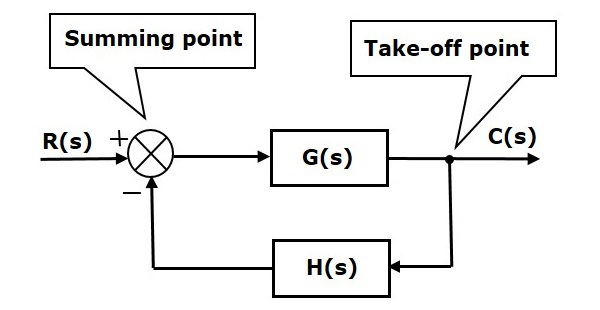
\includegraphics[width=6cm,0.5]{basic_block_diagram.jpg}
\end{center}
\end{frame}
\begin{frame}
Solution: Negative feedback system with G(s)=$\frac{1}{(s+1)(s+2)}$ ,H(s)=$\frac{s+\alpha}{s}$\break


\hspace{1.5cm} transfer function for negative feedback system  $\frac{C(s)}{R(s)}$=$\frac{G(s)}{1+G(s)H(s)}$\break

\hspace{3cm} $\frac{G(s)}{1+G(s)H(s)}$=$\frac{\frac{1}{(s+1)(s+2)}}{1+\frac{1}{(s+1)(s+2)}\frac{s+\alpha}{s}}$ \break

\hspace{3cm} transfer function = $\frac{s}{(s^3 +3s^2+ 3s+ \alpha)}$ \hfill \break
\end{frame}
\begin{frame}
we have to find value of $\alpha$ for which the poles of the system will be lying on imaginary axis.
 for determining the location of closed loop poles \break

 
 
 
 
 
 
 \hspace{3cm}        \polylongdiv{s^3+3s^2+3s}{}+ $\alpha$=0 \hfill \break

 \end{frame}
\begin{frame}

 Hence we can form the Routh’s array using characteristic polynomial  \hfill \break 
 
 \hspace{3cm} P(s)=\polylongdiv{s^3+3s^2+3s}{}+ $\alpha$ \hfill \break

    

  \hspace{3cm} \polylongdiv{s^3}{} \hspace{1cm} 1\hspace{1cm} 3\hspace{1cm} 0 \hfill \break
  
  \hspace{3cm} \polylongdiv{s^2}{} \hspace{1cm} 3\hspace{1cm} \alpha\hspace{1cm} 0 \hfill\break
  
  \hspace{3cm} \polylongdiv{s^1}{} \hspace{1cm} \frac{(9-\alpha)}{3} \hspace{0.5cm}0\hspace{1cm}0
  
  \hspace{3cm} \polylongdiv{s^0}{}\hspace{1cm} \alpha\hspace{1cm} \hspace{0.5cm}0\hspace{1cm}0\hfill \break
  \end{frame}
\begin{frame}
  If closed loop poles will be lying on imaginary axis, then the system will be marginally stable and the
conditions is satisfied by Routh’s array, if any complete row (except last) become zero.
 Having seen the first column of Routh’s array, poles will on imaginary axis, when \hfill\break
 
 \hspace{3cm}     $\frac{(9-\alpha)}{3}=0 \hfill \break
  
  \hspace{3cm}   Hence, \alpha=9
  
  \hspace{0.5cm} now put $\alpha$=9 in characteristic equation 
  now characteristic equation is P(s)=\polylongdiv{s^3+3s^2+3s+9}{}\hfill\break
  
  \hspace{1cm} poles are s= -3,j$\sqrt{3}$ ,-j$\sqrt{3}
  
  
\end{frame}

\end{document}
